\section{Results}
* Plenty of data~\cite{projectSpreadsheet}
* In terms of frame latency, lower values mean higher performance as frames are delivered more quickly
* The order of the legend in each graph is relative to the order which these conditions were tested, meaning the top one is the first one and the bottom one is the last one. 

\subsection{Overview of Search Space}
\begin{figure}[tbph]
    \centering
    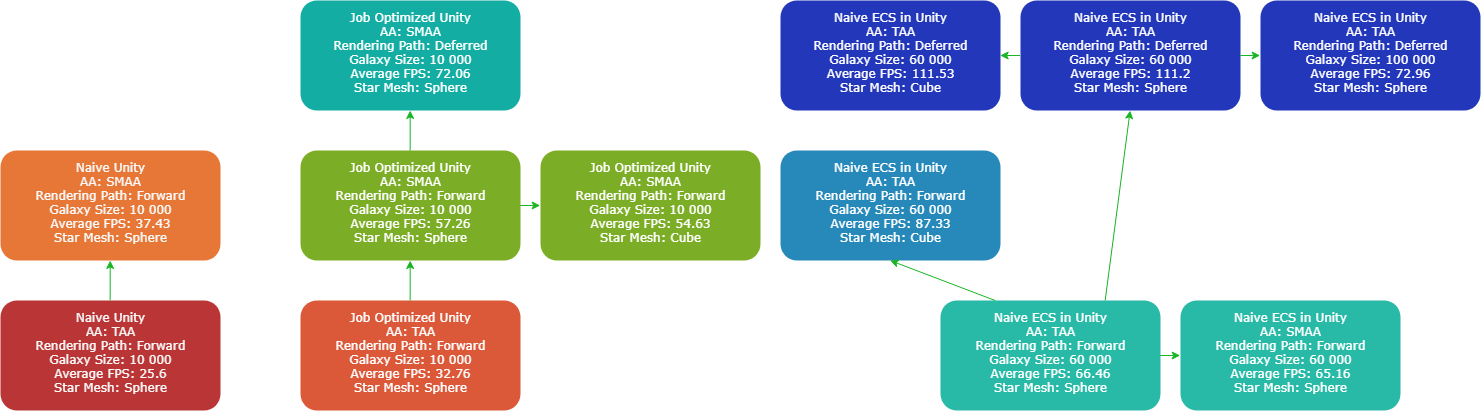
\includegraphics[width=1\textwidth]{Figures/SearchSpace.png}
    \caption[Optimisation Search Space And Combinations]{The space of optimisations that were measured}
    \label{fig:searchspace}
\end{figure}

* Figure~\ref{fig:searchspace}

\subsection{Naive Unity Tests}
\begin{figure}[!p]
    \centering
    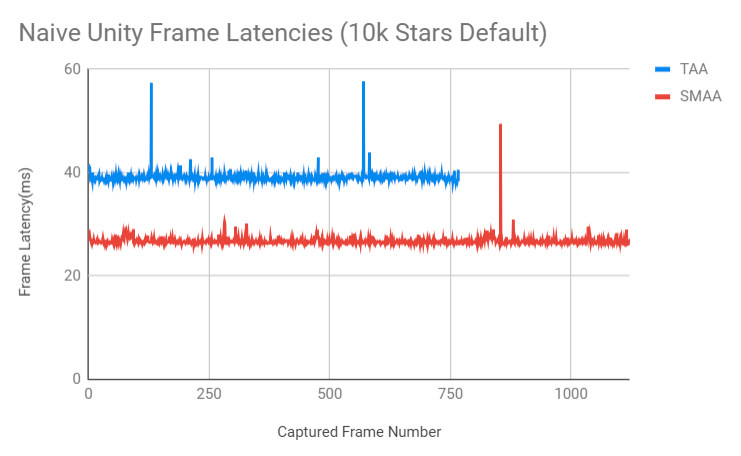
\includegraphics[width=1\textwidth]{Figures/naiveUnityLatencies.png}
    \caption[Combined Frame Latency Chart for Naive Unity Tests]{The combined chart of measured frame latencies for all naive Unity tests}
    \label{fig:naiveUnityLatency}
\end{figure}

* Video Link
* Figure~\ref{fig:naiveUnityLatency}
* Opting for SMAA as AA method yielded best performance/lowest frame latency here

\subsection{Job Optimised Unity Tests}
\begin{figure}[!p]
    \centering
    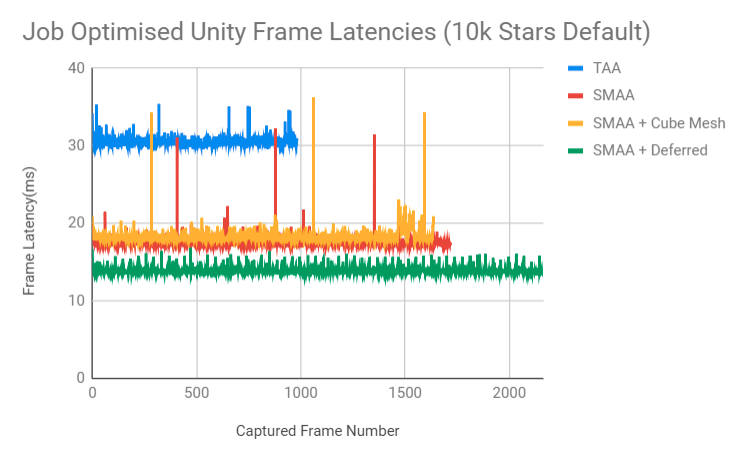
\includegraphics[width=1\textwidth]{Figures/jobOptimisedUnityLatencies.png}
    \caption[Combined Frame Latency Chart for Job Optimised Unity Tests]{The combined chart of measured frame latencies for all job optimised Unity tests}
    \label{fig:jobOptimisedUnityLatency}
\end{figure}

* Video Link
* Figure~\ref{fig:jobOptimisedUnityLatency}
* Similarly to Naive Unity, opting for SMAA instead of TAA generally improved performance. Using deferred instead of forward further improved performance, but not to the same degree as changing AA method.

\subsection{Naive ECS Tests}
\begin{figure}[!p]
    \centering
    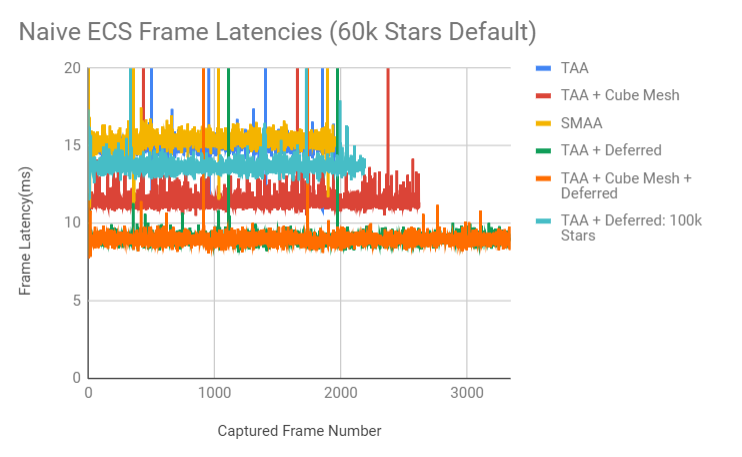
\includegraphics[width=1\textwidth]{Figures/naiveEcsLatencies.png}
    \caption[Combined Frame Latency Chart for Unity Tests]{The combined chart of measured frame latencies for all Naive ECS tests}
    \label{fig:naiveEcsUnityLatency}
\end{figure}

* Video Links
* Figure~\ref{fig:naiveEcsUnityLatency}
* performance is generally good for ECS
* Best performance was provided by TAA + deferred rendering
* Compared to the other two test cases, use of post processing AA did not appear to affect the results in a similar way. 
* A test case with 100k stars is included here to see the scalability of the best performing test

\subsection{Average framerate for all tests}
\begin{figure}[!p]
    \centering
    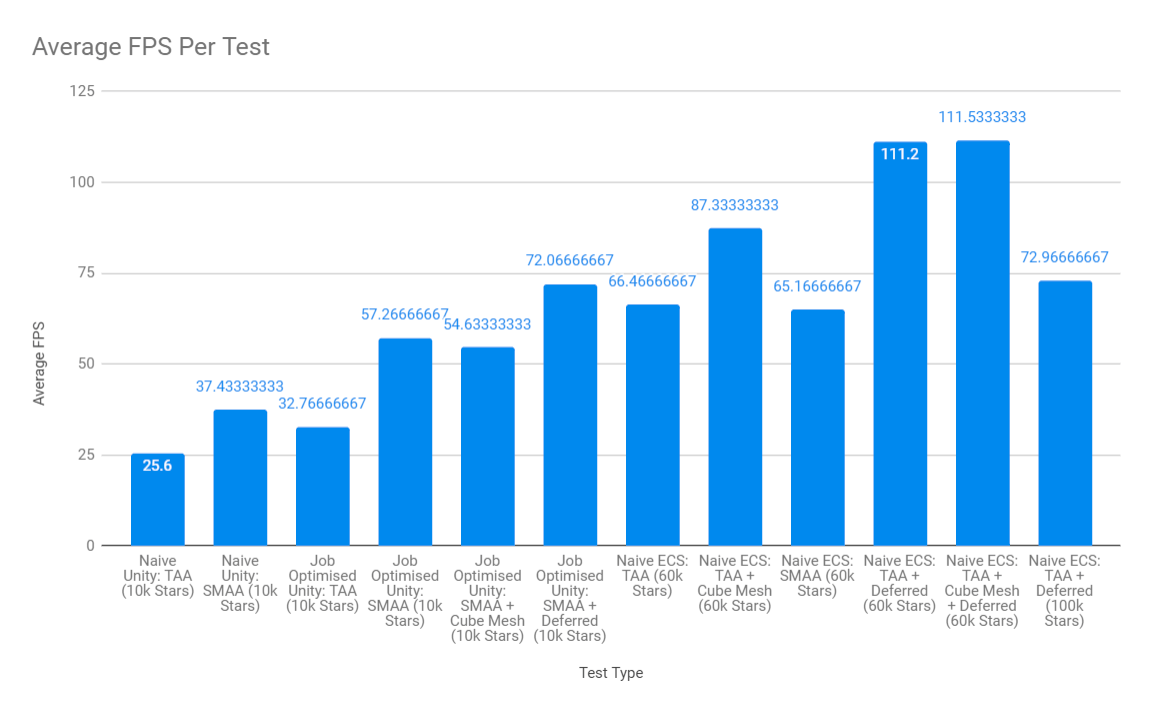
\includegraphics[width=1\textwidth]{Figures/averageFpsPerTest.png}
    \caption[Average Framerate Per Test]{The average framerate for all tests}
    \label{fig:averageFPS}
\end{figure}

* Figure~\ref{fig:averageFPS}
* Averages calculated by taking the total amount of recorded frames divided by 30 as it was the recording period.
* Taking into account that ECS by default consists of 60 000 stars the performance difference is rather large. 
* 100k stars in the TAA + Deferred case for ECS provided similar performance to the best performing Job optimised Unity case which was at 10k stars. 